\documentclass[a4]{article}
\usepackage[utf8]{inputenc}
\usepackage[french]{babel}
\usepackage{listings}
\usepackage{color}
\usepackage{graphicx}
\usepackage[T1]{fontenc}
\usepackage{pdfpages}
\usepackage{geometry}
\geometry{hmargin=2.5cm,vmargin=2.5cm}

\definecolor{mygreen}{rgb}{0,0.6,0}
\definecolor{mygray}{rgb}{0.5,0.5,0.5}
\definecolor{mymauve}{rgb}{0.58,0,0.82}

\lstset{
  backgroundcolor=\color{white},   % choose the background color; you must add \usepackage{color} or \usepackage{xcolor}
  basicstyle=\footnotesize,        % the size of the fonts that are used for the code
  breakatwhitespace=false,         % sets if automatic breaks should only happen at whitespace
  breaklines=true,                 % sets automatic line breaking
  captionpos=b,                    % sets the caption-position to bottom
  commentstyle=\color{mygreen},    % comment style
  deletekeywords={...},            % if you want to delete keywords from the given language
  escapeinside={\%*}{*)},          % if you want to add LaTeX within your code
  extendedchars=true,              % lets you use non-ASCII characters; for 8-bits encodings only, does not work with UTF-8
  frame=L,	                       % adds a frame around the code
  keepspaces=true,                 % keeps spaces in text, useful for keeping indentation of code (possibly needs columns=flexible)
  keywordstyle=\color{blue},       % keyword style
  language=C,                 	   % the language of the code
  otherkeywords={*,...},           % if you want to add more keywords to the set
  numbers=none,                    % where to put the line-numbers; possible values are (none, left, right)
  numbersep=5pt,                   % how far the line-numbers are from the code
  numberstyle=\tiny\color{mygray}, % the style that is used for the line-numbers
  rulecolor=\color{black},         % if not set, the frame-color may be changed on line-breaks within not-black text (e.g. comments (green here))
  showspaces=false,                % show spaces everywhere adding particular underscores; it overrides 'showstringspaces'
  showstringspaces=false,          % underline spaces within strings only
  showtabs=false,                  % show tabs within strings adding particular underscores
  stepnumber=2,                    % the step between two line-numbers. If it's 1, each line will be numbered
  stringstyle=\color{mymauve},     % string literal style
  tabsize=2,	                   % sets default tabsize to 2 spaces
  title=\lstname                   % show the filename of files included with \lstinputlisting; also try caption= instead of title
}
%gestion des caractères latins
\lstset{literate=
  {á}{{\'a}}1 {é}{{\'e}}1 {í}{{\'i}}1 {ó}{{\'o}}1 {ú}{{\'u}}1
  {Á}{{\'A}}1 {É}{{\'E}}1 {Í}{{\'I}}1 {Ó}{{\'O}}1 {Ú}{{\'U}}1
  {à}{{\`a}}1 {è}{{\`e}}1 {ì}{{\`i}}1 {ò}{{\`o}}1 {ù}{{\`u}}1
  {À}{{\`A}}1 {È}{{\'E}}1 {Ì}{{\`I}}1 {Ò}{{\`O}}1 {Ù}{{\`U}}1
  {ä}{{\"a}}1 {ë}{{\"e}}1 {ï}{{\"i}}1 {ö}{{\"o}}1 {ü}{{\"u}}1
  {Ä}{{\"A}}1 {Ë}{{\"E}}1 {Ï}{{\"I}}1 {Ö}{{\"O}}1 {Ü}{{\"U}}1
  {â}{{\^a}}1 {ê}{{\^e}}1 {î}{{\^i}}1 {ô}{{\^o}}1 {û}{{\^u}}1
  {Â}{{\^A}}1 {Ê}{{\^E}}1 {Î}{{\^I}}1 {Ô}{{\^O}}1 {Û}{{\^U}}1
  {œ}{{\oe}}1 {Œ}{{\OE}}1 {æ}{{\ae}}1 {Æ}{{\AE}}1 {ß}{{\ss}}1
  {ű}{{\H{u}}}1 {Ű}{{\H{U}}}1 {ő}{{\H{o}}}1 {Ő}{{\H{O}}}1
  {ç}{{\c c}}1 {Ç}{{\c C}}1 {ø}{{\o}}1 {å}{{\r a}}1 {Å}{{\r A}}1
  {€}{{\EUR}}1 {£}{{\pounds}}1
}
%definition d'un syle pour les documents text
\lstdefinestyle{txt}{
	frame=none,
	numbers=none,
	stringstyle=\color{black},
}

\begin{document}
	\title{\Huge{\textbf{Rapport Final}}}
	\author{Alabi Steve - Benyamna Younes - Capdenat Nicolas- \\
		Chouipe Thibaut - El Harti Zakaria - Lienhardt Florian \\ \\ \\
		Chef de projet : Benyamna Younes \\ \\ \\ 
		Sous la direction de Mme Kloul \\ \\ \\ \\
		Outil automatique de décryptage \\ \\ \\}
	\date{29 mai 2017}
		

	\begin{titlepage}
		\maketitle
		\vspace{20em}
		%\begin{center}
\includegraphics{logo_uvsq.jpg}\end{center}
	\end{titlepage}
	\section{Introduction}
Après avoir réalisé les charges et les spécifications, l'application Dcrypt est maintenant disponible et utilisable par le client. Ce rapport décrit les fonctionnalités de l'application, son architecture logiciel ainsi qu'une partie technique \\
Un manuel d'utilisation détaillé lui est fournit pour cela.
	\section{Objectif de l'application}
	Le but du projet est de developper un logiciel convivial de cryptanalyse pour tenter de décrypter un texte. Notre travail consiste a fournir un outil automatique d'aide au décryptage des fichiers/textes crypté par le chiffrement de Vigenère ou par  Substitution. L'utilisateur peut egalement crypter (avec V. ou S) ou plus simplement effectuer une analyse fréquentielle sur un texte.
	\section{Organigramme/explications}
			\underline{Interface graphique :}     \hspace{5cm}  \underline{Cryptage Substitution :}\\
			- bouton cryptage            \hspace{5.5cm}       -créer une clé aleatoirement\\
			- bouton decryptage         \hspace{5cm}        -crypter le message\\
			- bouton substitution\\
			- bouton Vigenère           \hspace{5.2cm}       \underline{Cryptage Vigenère :}\\
			- affichage de text(complet et partiel)  \hspace{2.2cm} -crypter le message\\
			- affichage pour la clé de substitution\\
			- bouton Francais(decryptage)   \hspace{3.5cm}     \underline{Decryptage Substitution :}\\
			- bouton Anglais(decryptage)    \hspace{3.5cm}     -decrypter le message\\
			- affichage pour l'analyse fréquentielle\\
			- charger un fichier text       \hspace{4.2cm}  \underline{Analyse fréquentielle :}\\
			- sauvegarder un fichier text     \hspace{3.8cm}  -analyse frequentielle sur text donné\\
			- créer un nouveau fichier text(resultats)\\
			- Demander clef de Vigenère\\
			
			
			\underline{Decryptage Vigenère :}\\
			-decrypter le message\\
			

			%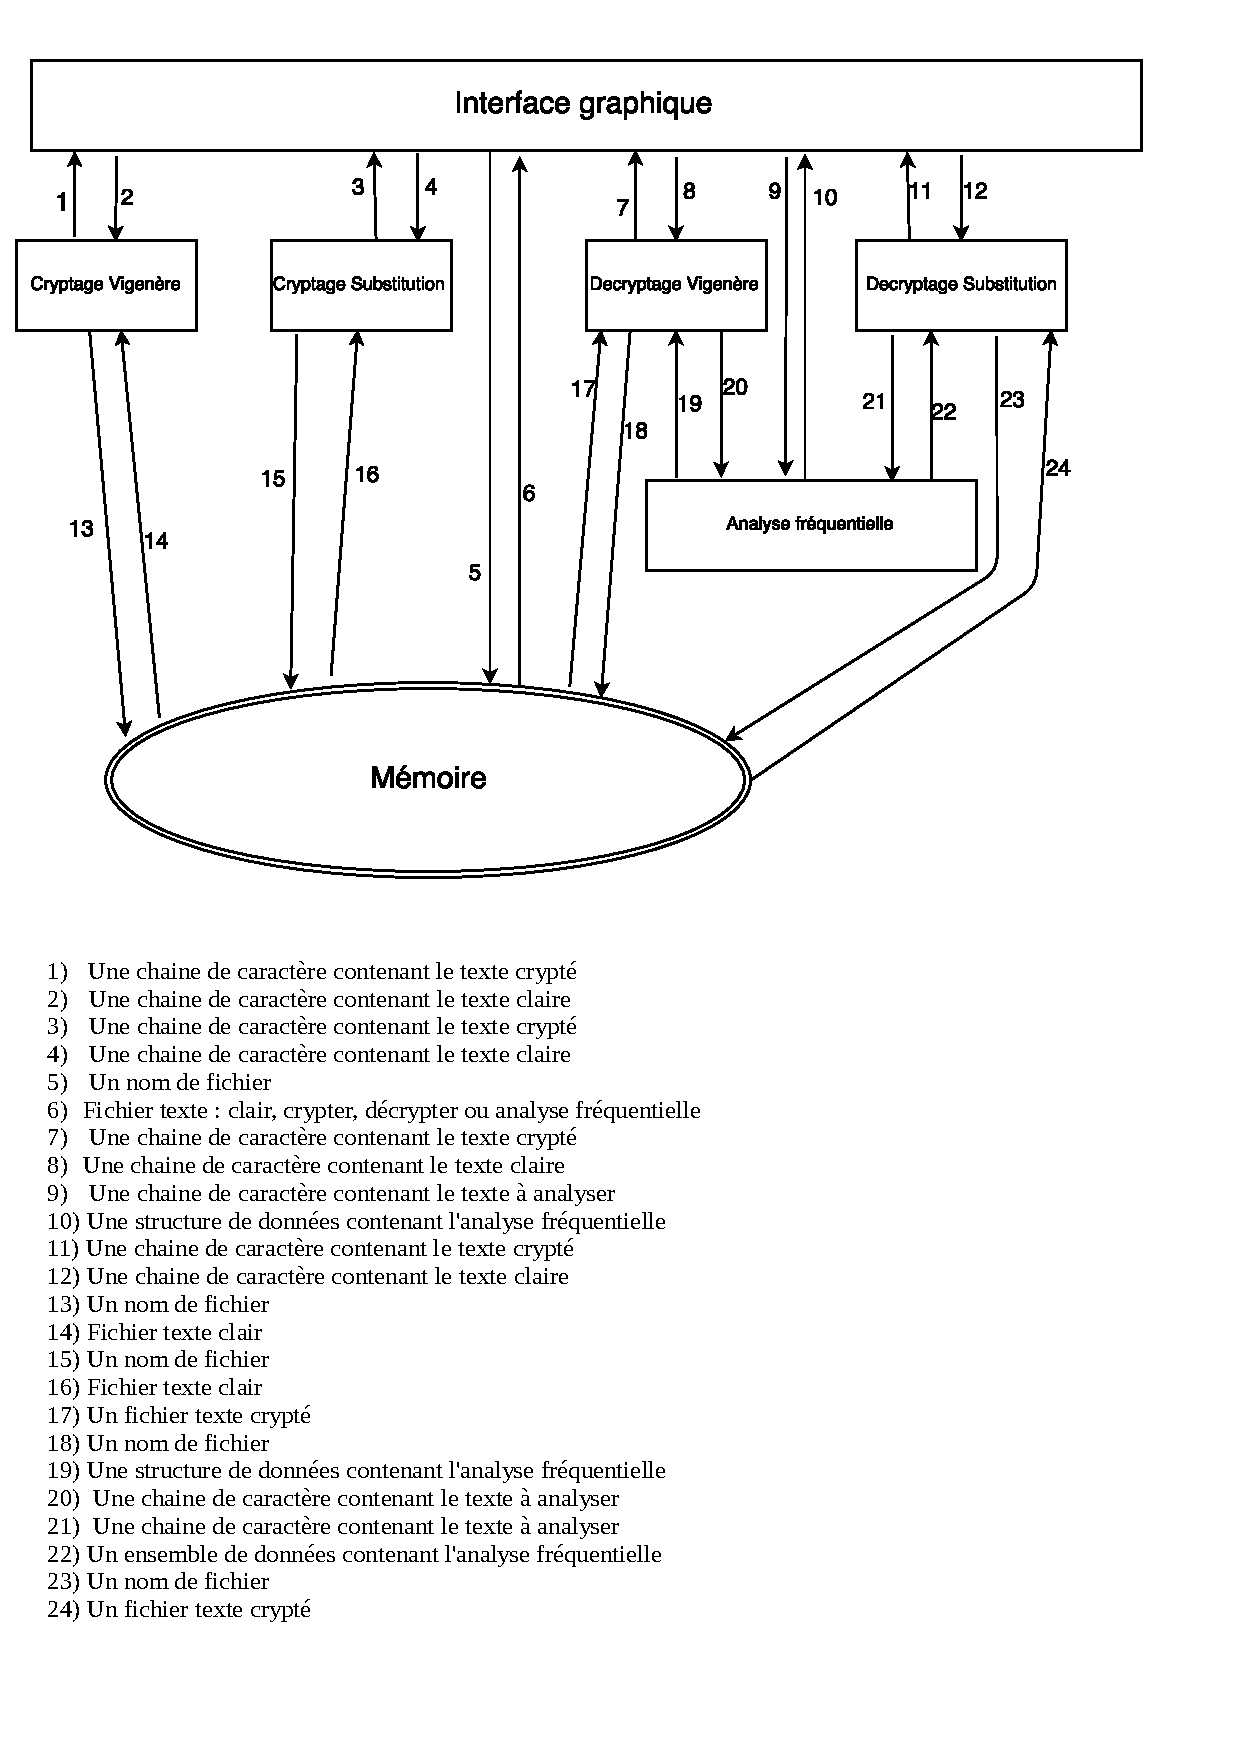
\includepdf[scale=0.65]{organ.pdf}
			
			il faut expilquer l'organigramme ICI
	\section{Language choisi et explication}
	Le developpement a ete realise en C. Ce choix a ete motive par  : \\
–
– 
-



La libraire gtk+ permet/ressources..

	\section{Partie technique}
		Vigenere: \\
		Itération manuel pour trouver la taille de la clé car le test de Kasiski se trompe souvent. \\
		Avec itération automatique : marche 1 fois sur 2 pour petite clé et peut lafficher en double (ex: clecle). \\
		Oui cela fonctionne pour la plupart des cas.\\
		Problème rencontrées avec Kasiski et l'hypothèse fait sur la taille de la clé.
		solution => itération manuel pour la taille. \\
		
		-est ce quelle fonctionne ? oui \\
		-quels sont les problemes/bugs rencontrees ? segfault..ect  \\
		-sont ils resolu ? si oui comment  \\
		-probleme specifications: dure, probleme, mal reussi, 1e fois..ect, plus grosse difficulté rencontrée  \\
		-Nous souhaitions avoir une application complète qui puisse tourner sur des ordinateurs 
de tout systeme d'exploitation et ce, sans pour autant qu’il ne
consomme trop de mémoire ou de temps processeur. 
		\subsection{tests et gestion des exceptions:}
		L’exactitude des resultats de l'analyse etant tres importante pour les clients, nous avons predefinis des tests
unitaires pour chaque module intervenant lors du decryptage. Ainsi, a chaque etape de la conception du logiciel
nous avons pu verifier que le calcul n’etait pas altere. 
		les tests permettent de voir comment le logiciel réagit lors de futurs améliorations.
		Utilisation de Cunit => Création d'un registre et d'une suite de tests unitaires.
		Création automatique d'un Summary(récapitulatif) des tests.
		rq : besoin de l'option -lcunit a rajouter a la compilation des tests.  
		
	\section{Organisation interne et affectation des taches}
	L'organisation de l'équipe est une chose importante pour le bon fonctionnement du
projet et le deroulement du codage, et est faite selon nos capacités et nos disponibilités.  \\
		-tableau des taches  \\
		L'organisation etant bonne et la cohesion du groupe certaine, la repartition et la mise en place d'un planning s'est faite naturellement et a été respectée.  \\
		La communication étant la clé d'un projet d'un projet en groupe, nous avons préféré nous reunir tres regulierement et travailler en face tous ensemble et ce quel que soit l'etape du projet.
		\subsection{Planning de developpement}
		Cette phase a constitue l’etape critique du projet, avec d’une part la decision de coder l’interface graphique
et d’autre part l’integration de tous les modules. Lors de cette phase, les modules ont connu leurs dernieres evolutions. \\
Avant de tester l’ensemble de l’application, nous avons dans un premier temps codé et
testé chaque fonction ou plutot module pour savoir si elles fonctionnaient séparément. \\
Nous les avons ensuite
réunies en les assemblant étapes par étapes pour construire l’application finale.  \\
--> en priorité : interface graphique commencé tres tot et analyse frequentielle pr tibo et flo \\
-bilan mi-projet \\
En evaluant les connaissances de chacun et en faisant un point regulierement sur nos taches respectives, cela a permis d'avancer efficacement et donc de realiser le projet.
	\section{comparaison lignes de code}
		estimation + nombre de vrai lignes (tableau) \\
		si fonction trop longue pk? et laquelle? \\
		
	
	\section{Conclusion}
	ameliorations + des choix a changer  \\
	=> Rajout d'un bouton "Recherche Intelligente" qui tente de trouver du premier coup la taille de clé.
	-critique du projet \\
	Ameliorations possibles futures: \\
	-permettre a l'utilisateur de rentrer des informations qui facilite la cryptanalyse un type de texte (poeme, roman..),\\
	une taille de clé, ..
	-plus de langues \\
	-plus de cryptage/decryptage \\
	
	Finalement, nous avons une version "1.0" de l’application. La majorité des fonctionnalités
de base ont été implémentées et fonctionnent correctement mais il existe quelques
améliorations qui pourraient aboutir véritablement à une version "2.0" vraiment intéressante. \\
Quelques améliorations pourraient être ajoutées :
-
- 
- 
- 
-
	
	
Ce projet d'une durée d'un semestre(et plus precisement de semaines) est réelle expérience.
Cela a été enrichissant d'un point de vue personnel ou collectif:
il nous a apporté beaucoup, tant au
niveau technique qu’en terme de gestion de projet.  \\  \\
Nous connaissons maintenant l'importance du decoupage d'un projet en plusieurs etapes: cahier des charges, specifications,codage..
C'est un projet en "conditions d'entreprise" qui nous servira dans le futur.
C’est la première fois que nous travaillons en groupe autant nombreux et sur un projet avec des caracteristiques bien définies. \\ \\
Nous sommes
globalement satisfaits de ce que nous avons réalisé.
 Au niveau de la gestion du projet en équipe, nous avons réussi à bien nous répartir les
tâches afin de réaliser nos objectifs dans les temps et l'ambiance générale du groupe était très
bonne. 
	
	
	
\end{document}
